\newpage
\hypertarget{rules tex}{}
\subsection{Tex Rules}
\texHeader


\begin{itemize}

\item[$\blacktriangleright$] You may have noticed that a \texttt{Rules} folder was automatically created when you created the TGG. As you can imagine, this is
where you'll need to place each rule. Create your first one by right-clicking on the folder, and navigating to ``New/TGG Rule.'' Name it
\texttt{BoxToDictionaryRule}.

\item[$\blacktriangleright$] The rule should immediately open in the editor, sectioned into four scopes - \texttt{source}, \texttt{correspondence},
\texttt{target}, and \texttt{constraints}. Each of these need to be implemented in order to create a valid rule.

\item[$\blacktriangleright$] First, lets create the key objects for the transformation. Assuming that this rule will be applied for the first time between two
objects (meaning there is no context to work with), you'll need to make sure each object variable is set to create. In the \texttt{source} scope, create
\texttt{box} of type \texttt{Box}. Similarily, create a \texttt{dictionary} of type \texttt{Dictionary} in the \texttt{target} scope. Your rule should now
resemble Fig.~\ref{}.

\begin{figure}[htbp]
\begin{center}
  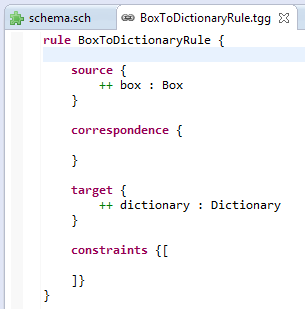
\includegraphics[width=0.5\textwidth]{eclipse_startRule}
  \caption{figureCaption}
  \label{fig:textSourceRule}
\end{center}
\end{figure}

\item[$\blacktriangleright$] Now we create our first TGG Correspondence link between these elements! In the \texttt{correspondence} scope, enter 
\syntax{++ box <- boxToDictionary : BoxToDictionary -> dictionary}
Note that the structure of this statement creates \emph{one} link, named \texttt{boxToDictionary}, of type \texttt{BoxToDictionary} (which we delcared in the
schema), that goes forward from \texttt{box} to \texttt{dictionary}, and backwards from \texttt{dictionary} to \texttt{box}.

\item[$\blacktriangleright$] This is great work so far, except if the transformation was to be run using this rule-as is, we would simply be creating these
objects with empty attributes. Let's try connecting the \texttt{name} of \texttt{box} to the \texttt{title} of the \texttt{dictionary} with an \emph{attribute
constraint}. Attribute constraints in TGG rules provide a bidirectional and high level solution for attribute manipulations.

\item[$\blacktriangleright$] Under the \texttt{constraints} scope, create an \texttt{equals} constraint via\footnote{Remember, each of these EAttributes were
declared in the appropriate EClass}
\syntax{eq(box.name, dictionary.title)}
Your rule should now resemble Fig.~\ref{fig:ruleBasic}.

\begin{figure}[htbp]
\begin{center}
  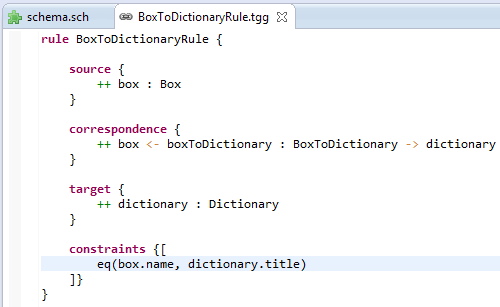
\includegraphics[width=0.8\textwidth]{eclipse_ruleBasic}
  \caption{figureCaption}
  \label{fig:ruleBasic}
\end{center}
\end{figure}

\item[$\blacktriangleright$] In an effort to have a tangible result, lets give our \texttt{box} a proper name, so that when we run this rule later, we'll be
able to see it assigned to the dictionary. Go to ``LearningBoxLanguage/instances'' and open \texttt{Box.xmi}. Double click \texttt{Box} until the
\texttt{Properties} tab activates below the editor, and update the \texttt{Name} attribute with any name you like.

% But, we still need to create the intial structure of our learning box. we've declared it, but haven't put anything in it. In contrast.. (pg 21)

\item[$\blacktriangleright$] Returning to \texttt{BoxToDictionaryRule}, in order to complete our TGG Rule, we still need to create the structure of the learning
box that would result from executing the \emph{backwards} transformation, from \texttt{dictionary} to \texttt{box}. In contrast to how every \emph{Entry} in a
\texttt{Dictionary} are simply contained within in, each \texttt{Card} in a \texttt{Box} is sorted into different \texttt{Partition}s. In the object variable
scrop for \texttt{box}, create \texttt{partition0}, \texttt{partitio1}, and \texttt{partition2}, each of type \texttt{Partition}. Your workspace should now
resemble Fig.~\ref{fig:firstReferences}.

\begin{figure}[htbp]
\begin{center}
  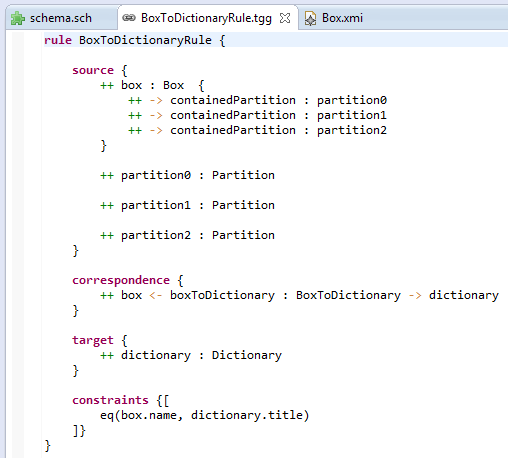
\includegraphics[width=0.8\textwidth]{eclipse_ruleContainedReferences}
  \caption{figureCaption}
  \label{fig:firstReferences}
\end{center}
\end{figure}

\item[$\blacktriangleright$] To complete each \texttt{partition} structure, we also need to set up the movement references as according to the Leitner Box
Rules -- if a card is guessed wrong, it will always be returned to the very first partition, no matter how far along it is. Conversely, if a card if guessed
correctly, it moves to the next partition in the sequence.\footnote{Read the introduction to Part II to review the rules and motivation behind our LeitnersBox}
Create the appropriate \texttt{previous} and \texttt{next} link variables for each \texttt{partition} until your workspace resembles
Fig.~\ref{fig:allReferences}.

\begin{figure}[htbp]
\begin{center}
  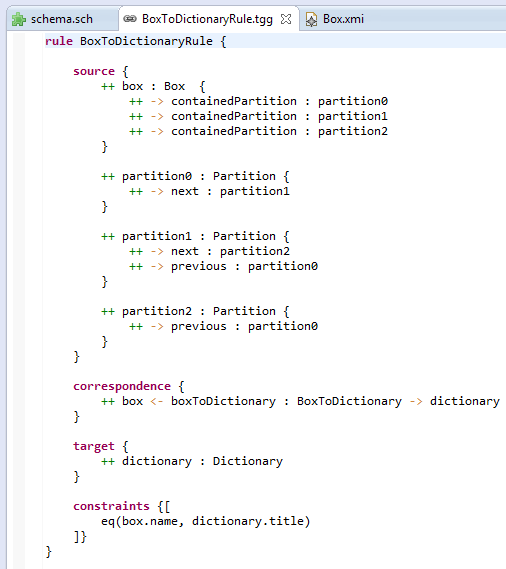
\includegraphics[width=0.8\textwidth]{eclipse_allReferences}
  \caption{figureCaption}
  \label{fig:allReferences}
\end{center}
\end{figure}

\end{itemize}

Fantastic work! Your first TGG rule is complete! This rule is able to transform a \texttt{box} into a \texttt{dictionary} and vice-versa. Unfortunately, it will
only be able to handle completely \emph{empty} boxes and dictionaries -- you can see that we haven't provided additional handling for \texttt{Card} or
\texttt{Entry} items.

If you're in a hurry, feel free to jump ahead to Section 4: TGGs in Action to execute this rule. Otherwise, the next rule we create will integrate itself with
\texttt{BoxToDictionaryRule} to increase its functionality. 


\begin{itemize} 

\item[$\blacktriangleright$] Analogusly to how you began the previous rule, create an \emph{Integration Class} called \texttt{CardToEntry} with a \texttt{Card}
source and \texttt{Entry} target. Your updated \texttt{Schema} should now resemble Fig.~\ref{fig:updatedSchema}.

\begin{figure}[htbp]
\begin{center}
  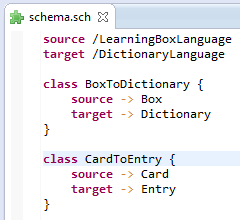
\includegraphics[width=0.4\textwidth]{eclipse_updatedSchema}
  \caption{figureCaption}
  \label{fig:updatedSchema}
\end{center}
\end{figure}

\item[$\blacktriangleright$] Right click on the \texttt{Rules} folder again, and create the TGG \texttt{CardToEntryRule}.

One of the key differences between this rule and the last is that this rule will only be invoked within a certain context i.e.,
this will only be used if a preexisting \texttt{partition} has \texttt{card} elements that need to be transformed into entires in an established
\texttt{dictionary}. In terms of MOSl, this means there will be both 'black' and 'green' elements.

\item[$\blacktriangleright$] To begin, create three object variables in the \texttt{source} scope: \texttt{box}, \texttt{partition0}, and \texttt{card}. Which
ones are already known from the context? Which element still needs to be made? Your rule should resemble Fig.~\ref{fig:c2eRuleSource}.

\begin{figure}[htbp]
\begin{center}
  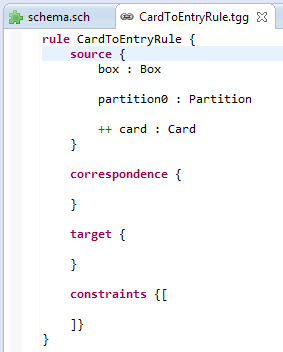
\includegraphics[width=0.4\textwidth]{eclipse_sourceOVs}
  \caption{figureCaption}
  \label{fig:c2eRuleSource}
\end{center}
\end{figure}

\item[$\blacktriangleright$] Next, lets set the \texttt{target}. Declare \texttt{dictionary : Dictionary}, and \texttt{++ entry : Entry}.

\item[$\blacktriangleright$] Now we have to fill in the \texttt{correspondence} scope. We need to first confirm the original link, then create a second one
between \texttt{card} and \texttt{entry} with the new correspondence type from our updated schema. Your workspace should resemble Fig.~\ref{fig:c2etargetCorresp}

\begin{figure}[htbp]
\begin{center}
  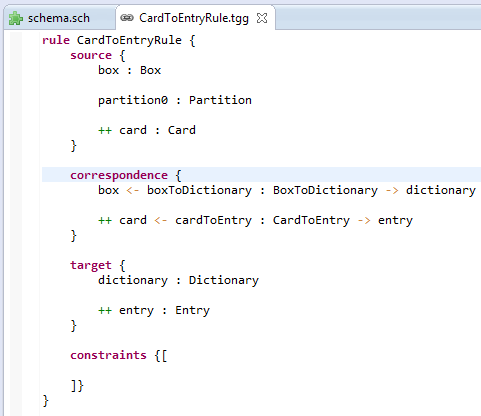
\includegraphics[width=0.8\textwidth]{eclipse_secondRuleStructured}
  \caption{figureCaption}
  \label{fig:c2etargetCorresp}
\end{center}
\end{figure}

\item[$\blacktriangleright$] Finally, let's make sure each transformation is able to access the \texttt{card} and \texttt{entry} contents. Complete your object
variable scopes until your rule matches Fig.~\ref{fig:c2eAllReferences}. If you're having trouble remembering the name of the relevant reference (from the
metamodel), feel free to open the appropriate \texttt{eclass} to find out what applies. Alternatively, eMoflon's type completion can help you here as well --
just press \texttt{ctrl + space} after writing \texttt{->} for a list of available link variables for that class.

\begin{figure}[htbp]
\begin{center}
  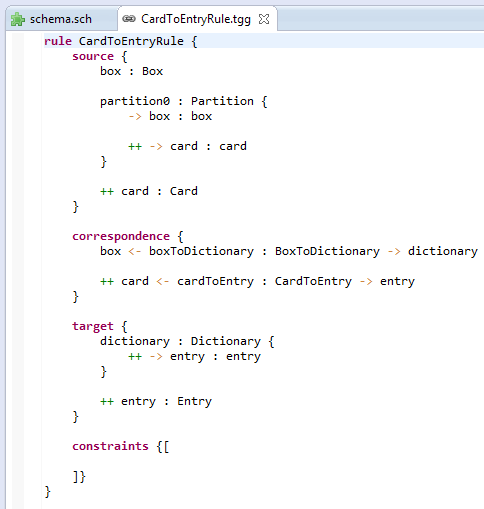
\includegraphics[width=0.8\textwidth]{eclipse_c2eAllReferences}
  \caption{figureCaption}
  \label{fig:c2eAllReferences}
\end{center}
\end{figure}

\item[$\blacktriangleright$] With each element now accessbile, we can update our \texttt{constraints}. Unlike the object variables, we don't need to re-declare
constraints from the previous rule. Instead, we need to create three strictly related to the contents of each \texttt{card} and \texttt{entry}:
(1) We want to 
(2) Do the same thing for ``Answer''
(3) Given that they all mean the same thing, we want to cocatnate \texttt{word}, \texttt{meaning}, and \texttt{entry.content}.

\item[$\blacktriangleright$] Your rule should now resemble Fig.~\ref{fig:contentConstraints}.

\begin{figure}[htbp]
\begin{center}
  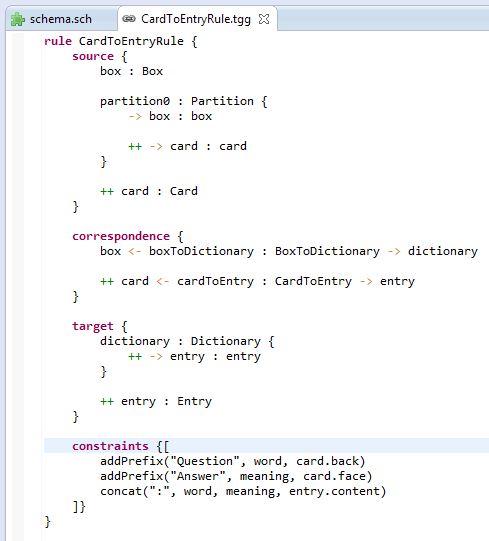
\includegraphics[width=0.8\textwidth]{eclipse_contentConstraints}
  \caption{figureCaption}
  \label{fig:contentConstraints}
\end{center}
\end{figure}

Let's add \emph{one} more constraint. Given that we have three partitions, and three difficulty levels for each \texttt{Entry}, why don't we have the
transformation assign a level based on whatever partition a \texttt{card} is found in? Hard cards, for example, are more likely to be found in the first
partition due to always being guessed wrong, so let's create a constraint that will make \emph{any} card found there \texttt{advanced}. As you can imagine,
there is no specific constraint existing in eMoflon to manage this -- we must create our own constraint.

\item[$\blacktriangleright$] Specify the rule within the \texttt{contraints} scope via: \syntax{indexToLevel[BB,BF,FB](EInt, EString)}

\item[$\blacktriangleright$] Now you can invoke your rule via: \texttt{indexToLevel(partition0.index, entry.level)}. Your completed rule should now resemble
Fig.~\ref{fig:c2eDone}.

\begin{figure}[htbp]
\begin{center}
  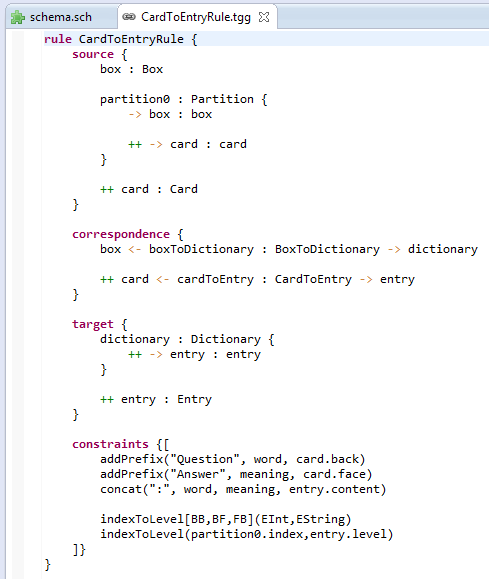
\includegraphics[width=0.8\textwidth]{eclipse_completedCardToEntryRule}
  \caption{figureCaption}
  \label{fig:c2eDone}
\end{center}
\end{figure}

\item[$\blacktriangleright$] Awesome work! If you haven't already, save the file and confirm the MOSL parser hasn't raised any errors, press
\texttt{``Build (Without Cleaning)''}, and admire your TGG transformation rules. 

\end{itemize}
